%!TEX TS-program = xelatex
%!TEX root = ../../maxwell2018thesis.tex

\chapter[Discussion and Future Work]{Discussion and Future Work}\label{chap:conclusions}
The final chapter of this thesis summarises and discusses the results reported in this thesis. In particular, we emphasise the impact of our findings on~\gls{acr:ir} and~\gls{acr:iir} research, as well as outlining several potential future research directions.

\section{Thesis Summary}\label{sec:conclusions:summary}
In this thesis, we examined how stopping behaviours vary under different search contexts. In particular, we conducted and reported on two user studies under the domain of news search, examining how~\raisebox{-.2\height}{
\includegraphics[height=5mm]{figures/ch2-point1.pdf}} result summary lengths and~\raisebox{-.2\height}{
\includegraphics[height=5mm]{figures/ch2-point2.pdf}} a variation of search tasks, goals and retrieval systems affected search behaviours. A total of eight different interfaces and conditions were used to examine how behaviours vary -- as summarised in Table~\ref{tbl:conclusion_cond_interface_summary}.

\begin{table}[t!]
    \caption[Summary of experimental interfaces and conditions]{A summary table of the different experimental interfaces and conditions that were trialled. These are based upon the work reported in Chapters~\ref{chap:snippets} and~\ref{chap:diversity}. In total, eight different experimental interfaces and conditioned were employed, considering different result summary lengths, systems and tasks.}
    \label{tbl:conclusion_cond_interface_summary}
    \renewcommand{\arraystretch}{1.8}
    \begin{center}
    \begin{tabulary}{\textwidth}{L{0.4cm}@{\CS}L{3.2cm}@{\CS}D{3.51cm}@{\CS}D{3.51cm}@{\CS}D{3.51cm}@{\CS}}
        & & \lbluecell \textbf{Summary Length} & \lbluecell \textbf{System} & \lbluecell \textbf{Task} \\
        
        \RS \multirow{4}{*}{\rotatebox{90}{\hspace*{-4mm}\textbf{Chapter~\ref{chap:snippets}}}} & \lbluecell\textbf{T0} & \cell \small{Title only} & \cell \small{\blueboxbold{ND} (Non Div.)} & \cell \small{\darkblueboxbold{AD} (Ad-hoc)}\\
        \RS & \lbluecell\textbf{T1} & \cell \small{Title + 1 snippet} & \cell \small{\blueboxbold{ND} (Non Div.)} & \cell \small{\darkblueboxbold{AD} (Ad-hoc)}\\
        \RS & \lbluecell\textbf{T2} & \cell \small{Title + 2 snippets} & \cell \small{\blueboxbold{ND} (Non Div.)} & \cell \small{\darkblueboxbold{AD} (Ad-hoc)}\\
        \RS & \lbluecell\textbf{T4} & \cell \small{Title + 4 snippets} & \cell \small{\blueboxbold{ND} (Non Div.)} & \cell \small{\darkblueboxbold{AD} (Ad-hoc)}\\
        
        \RS\RS\RS \multirow{4}{*}{\rotatebox{90}{\hspace*{-4mm}\textbf{Chapter~\ref{chap:diversity}}}} & \lbluecell\textbf{D-AS} & \cell \small{Title + 2 snippets} & \cell \small{\blueboxbold{D} (Div.)} & \cell \small{\darkblueboxbold{AS} (Aspectual)}\\
        \RS & \lbluecell\textbf{ND-AS} & \cell \small{Title + 2 snippets} & \cell \small{\blueboxbold{ND} (Non Div.)} & \cell \small{\darkblueboxbold{AS} (Aspectual)}\\
        \RS & \lbluecell\textbf{D-AD} & \cell \small{Title + 2 snippets} & \cell \small{\blueboxbold{D} (Div.)} & \cell \small{\darkblueboxbold{AD} (Ad-hoc)}\\
        \RS & \lbluecell\textbf{ND-AD} & \cell \small{Title + 2 snippets} & \cell \small{\blueboxbold{ND} (Non Div.)} & \cell \small{\darkblueboxbold{AD} (Ad-hoc)}\\
        
    \end{tabulary}
    \end{center}
\end{table}

From the first user study reported in Chapter~\ref{chap:snippets}, results showed that as result summary lengths increased (from \blueboxbold{T0}$\rightarrow$\blueboxbold{T4}), searchers became more confident in the decisions they took pertaining to the relevance of documents encountered. However, this was not reflected empirically; their accuracy in identifying relevant content did not improve with longer result summaries. In terms of stopping behaviours, a downward trend was observed. As the length of result summaries increased, subjects examined to shallower depths per query -- an intuitive result, given the increased examination times required for longer summaries.

Considering variations of tasks, goals and systems as reported in Chapter~\ref{chap:diversity}, we found that when using diversified system \blueboxbold{D} (i.e. BM25 and XQuAD~\citep{santos2010query_reformulations_diversification}), subjects issued more queries, and stopped at comparatively shallower depths per query. This was in comparison to non-diversified system \blueboxbold{ND} (i.e. BM25 baseline), where subjects reported feeling less confident about their decisions. Despite the significant differences we observed with regard to how the two systems performed, few significant differences were observed when examining changes in searcher behaviours. Most subjects reported difficulty in identifying differences in performance between the two systems.

Analysis of interaction data from these user studies was then used to ground an extensive set of simulations of interaction. These simulations were designed to test a total of twelve individual stopping strategies, derived from a variety of stopping heuristics\footnote{Stopping heuristics for example considered a searcher's tolerance to non-relevance, or their \emph{frustration} with observing non-relevant content~\citep{kraft1979stopping_rules}.} and~\gls{acr:ir} measures having been defined in the literature. Our novel technique of cataloguing, together with the subsequent operationalisation of them into stopping strategies provided an answer to \darkblueboxbold{HL-RQ2}. We then tested the overall performance and how closely the simulations matched up to real-world searcher behaviours (across the eight experimental interfaces and conditions). In turn, this allowed us to provide answers to both \darkblueboxbold{HL-RQ3a} and \darkblueboxbold{HL-RQ3b}. The simulations were based upon the~\glsfirst{acr:csm}, an updated, high-level conceptual model of the search process. By incorporating a new~\gls{acr:serp} level stopping decision point into the~\gls{acr:csm}, complete with subsequent empirical evaluation (as presented in Chapter~\ref{chap:serp}), we could then provide an answer to \darkblueboxbold{HL-RQ1}.

Results show that when enabled, the new~\gls{acr:serp} stopping decision point led to significant improvements over the baseline implementation, with consistent improvements in overall performance (measured in~\gls{acr:cg}) reported across a range of experimental conditions, interfaces and stopping strategies. Improvements in approximations of real-world searcher stopping behaviours were also achieved -- although, however, statistical significance for these improvements was not obtained. Overall, these results provide compelling evidence for \darkblueboxbold{HL-RQ1}, and also demonstrate a promising direction for future research in developing our understanding of the search process.

With respect to our simulated analyses of individual stopping strategies, we found several stopping strategies offered high levels of~\gls{acr:cg}, and good approximations toward actual searcher stopping behaviours. For example, we found that with increased result summary length, \blueboxbold{SS11-COMB} consistently offered the best performance, with \blueboxbold{SS1-FIX} and \blueboxbold{SS4-SAT} offering the best real-world searcher approximations. Furthermore, \blueboxbold{SS5-COMB} offered the best level of~\gls{acr:cg} within the second user study, while \blueboxbold{SS1-FIX} offered the best level of performance across condition \dualbluebox{ND}{AD}. On the contrary, however, \blueboxbold{SS1-FIX} and \blueboxbold{SS10-RELTIME} yielded the lowest MSE values. However, despite several strategies performing well, no single strategy clearly emerged as offering significantly improved levels of performance or approximations when acting alone. On the contrary, several more complex stopping strategies offered poorer performance, such as \blueboxbold{SS6-DT} and \blueboxbold{SS7-DKL}. This was a common theme in our results: simple and combination-based stopping strategies generally provided the highest levels of performance. This includes the fixed-depth stopping strategy, \blueboxbold{SS1-FIX}, which, counter to our intuition, consistently performed well.

\section{Discussion}\label{sec:conclusions:discussion}
From the analysis of our simulations of interaction, a number of novel, interesting areas of discussion were revealed. In this section, we discuss our findings with an emphasis on examining the stopping strategies that were trialled. In particular, our discussion is guided by our four high-level research questions. We repeat these below.

\begin{itemize}
    \item{\darkblueboxbold{HL-RQ1} How can we improve searcher models to incorporate different stopping decision points?}
    \item{\darkblueboxbold{HL-RQ2} Given the stopping heuristics defined in the literature, how can we encode these heuristics into a series of operationalised, programmable stopping strategies that can be subsequently incorporated into the searcher model and be evaluated?}
    \item{\darkblueboxbold{HL-RQ3a} Given the aforementioned operationalised stopping strategies, how well does each one perform?}
    \item{\darkblueboxbold{HL-RQ3b} How closely do the operationalised stopping strategies compare to the actual stopping behaviours of real-world searchers?}
\end{itemize}

With these research questions pertaining to the simulations of interaction (along with the implemented stopping strategies), in-depth discussion of our user studies can be found in Sections~\ref{chap:snippets:user:discussion} on page~\pageref{chap:snippets:user:discussion} and~\ref{sec:diversity:users:discussion} on page~\pageref{sec:diversity:users:discussion}. However, we do briefly touch on summarising statements relating to searcher behaviours in Section~\ref{sec:conclusions:discussion:behaviours}.

\subsection{Searcher Models and Realism}\label{sec:conclusions:discussion:realism}
Work in this thesis has reported advancements to modelling the~\gls{acr:iir} process -- particularly with the inclusion of the new~\gls{acr:serp} level stopping decision point. The inclusion of the new stopping decision point led to significant improvements in terms of the level of~\gls{acr:cg} that could be attained, together with improved approximations of real-world behaviours.

However, these significant improvements from the \blueboxbold{Always} baseline (as reported in Chapter~\ref{chap:serp}) were only achieved with the \blueboxbold{Perfect} implementation. This is a limitation, as the implementation relied upon access to the~\gls{acr:trec} QRELs in order for the impression to be determined. While improvements in performance and approximations were noted with the \blueboxbold{Average} implementation, these changes did not achieve a significant level of improved performance. We discuss this limitation of our simulations later in Section~\ref{sec:conclusions:discussion:simulations}.

Of course, attaining access to the \emph{gold standard} is wholly unrealistic. However, the present study demonstrates the \emph{maximum performance} that can be reached with the inclusion of this new stopping decision point. The observed improvements demonstrate that more realistic simulations of interaction may be produced. With further work examining the proximal cues that searchers observe when forming an initial impression of the~\gls{acr:serp}, incorporating these findings into future simulations of interaction would arguably make them even more realistic.

\subsection{Stopping Strategy Operationalisation}\label{sec:conclusions:discussion:strategies}
In general, findings across all interfaces and conditions trialled demonstrated that simple stopping strategies tended to yield better performance, and matched better with real-world searcher stopping behaviours. Stopping strategies \blueboxbold{SS2-NT}, \blueboxbold{SS3-NC}, \blueboxbold{SS4-SAT}, \blueboxbold{SS9-TIME} and \blueboxbold{SS10-RELTIME} for example performed and approximated well. We consider these to be simple in the sense that the stopping criterion that they each encoded was straightforward to implement and subsequently measure. Examples included the consideration of aspects such as the number of non-relevant documents encountered, or the elapsed time spent searching since query issuance.

In contrast, findings also demonstrated that the more complex stopping strategies tended to perform worse. They consistently offered poorer performance and approximations. Complexity was again denoted by the criterion/criteria that were considered by each strategy, with more complex computations required in order to determine when the simulated searcher should stop. Given these general findings, \emph{why did the more complex stopping strategies perform and approximate worse on average?} The present section of the discussion focuses primarily on this question, considering the difference-based strategies \blueboxbold{SS6-DT} and \blueboxbold{SS7-DKL}, the~\gls{acr:ift}-based strategy \blueboxbold{SS8-IFT}, and the~\gls{acr:rbp}-based strategy \blueboxbold{SS12-RBP}. We also discuss the importance of more performant stopping strategies, such as \blueboxbold{SS5-COMB} and \blueboxbold{SS11-COMB}.

\blueboxheader{Difference Stopping Strategies}
Considering \blueboxbold{SS6-DT} and \blueboxbold{SS7-DKL}, we hypothesise that the performance of issued queries may be having an effect on the way in which these strategies perform. In other words, the stopping strategies \emph{may not be very robust} to varying levels of query performance. Recall that for our \emph{what-if} performance runs, we employed an interleaved querying strategy, \blueboxbold{QS13}.\footnote{Refer to Section~\ref{sec:method:simulation:grounding:querying} on page~\pageref{sec:method:simulation:grounding:querying} for additional information on how the querying strategy was implemented.} With this strategy, single term and three term queries were interleaved. From empirical evidence, it was shown that single term queries offered poor performance (in terms of $P@k$) when compared to three term queries -- single term queries offered higher levels of diversity compared to the three term queries.\footnote{For example, consider the queries \texttt{`piracy'} and \texttt{`piracy china sea'}. The first single term query returned a majority of documents pertaining to software piracy, along with piracy at sea. In contrast, the three term query returned a majority of its matched documents to instances of piracy on the South China Sea, relevant to the~\gls{acr:trec} piracy topic.} As such, using a fixed threshold across queries of varying performance would not necessarily make sense. A low threshold for \blueboxbold{SS6-DT} and \blueboxbold{SS7-DKL} would mean that searchers would stop too early for single term queries, and examine too deeply for three term queries. A higher threshold would mean that searchers would browse too deep for single and three term queries. For example, this means that a low threshold would be too stringent for single term queries, and suggests that poor levels of gain would be achieved.

\begin{figure}[t!]
    \centering
    \resizebox{1\hsize}{!}{
    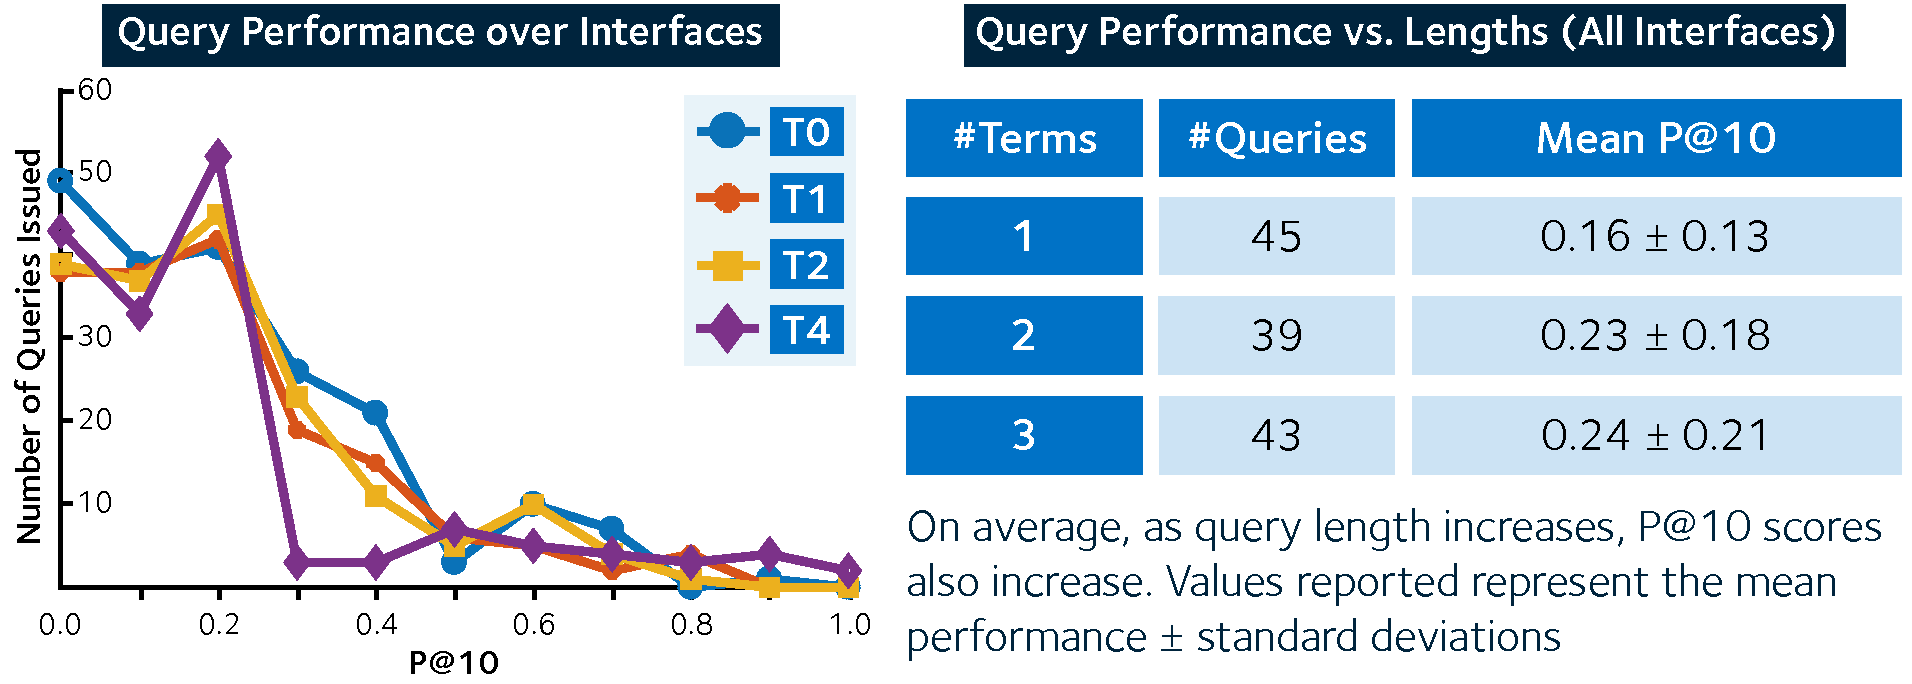
\includegraphics{figures/ch10-queryperf.pdf}}
    \caption[Query performance by real-world subjects]{Plot demonstrating the performance of queries (\genericblack{P@10}) across the four experimental interfaces trialled in the user study we report on in Chapter~\ref{chap:snippets}. On the right, a table highlights the varying levels of performance (averaged over all four experimental interfaces) in relation to query term lengths. As query term length increases, so too does the mean P@10 score. Similar findings were observed for the study reported in Chapter~\ref{chap:diversity}.}
    \label{fig:query_performance_ch7}
\end{figure}

As such, we hypothesise that for stopping strategies based upon the difference-based heuristic, thresholds should likely be query specific -- perhaps dependent upon the length of the query issued. Given queries issued by the real-world subjects in Chapter~\ref{chap:snippets}, we also observed a large variation in performance for the queries that were issued. We report this in Figure~\ref{fig:query_performance_ch7}, with a plot showing the number of queries issued across each of the four interfaces, plotted against the performance of the queries. A table also provides evidence to support our hypothesis, showing that as the number of terms in the queries increased, so too did the mean level of query performance. Similar findings were observed in the user study reported in Chapter~\ref{chap:diversity}.

\blueboxheader{\gls{acr:ift} Stopping Strategy}
Next, we consider the poor performance and approximations afforded by \blueboxbold{SS8-IFT}. Evidence has shown that~\gls{acr:ift} has been proven to be good at predicting search behaviours~\citep{ong2017scent_behaviour, azzopardi2018cwl}. In Section~\ref{sec:diversity:users:results:ift} on page~\pageref{sec:diversity:users:results:ift}, we demonstrated that our~\gls{acr:ift}-based hypotheses matched closely to empirical evidence. So, why did \blueboxbold{SS8-IFT} consistently offer poorer performance and approximations when compared to more simplistic stopping strategies? We hypothesise that this comparative lack of performance can be attributed to how the \emph{rate of gain} was operationalised, which serves as the stopping criterion for \blueboxbold{SS8-IFT}. This is an inherently difficult value to compute, with limitations relating to the rate of gain considered from two angles:

\begin{itemize}
    \item[\raisebox{-.2\height}{
\includegraphics[height=5mm]{figures/ch2-point1.pdf}}]{the \emph{per-topic} rate of gain; and}
    \item[\raisebox{-.2\height}{
\includegraphics[height=5mm]{figures/ch2-point2.pdf}}]{\emph{how the rate of gain is estimated} by searchers in the first instance.}
\end{itemize}

\begin{figure}[t!]
    \centering
    \resizebox{1\hsize}{!}{
    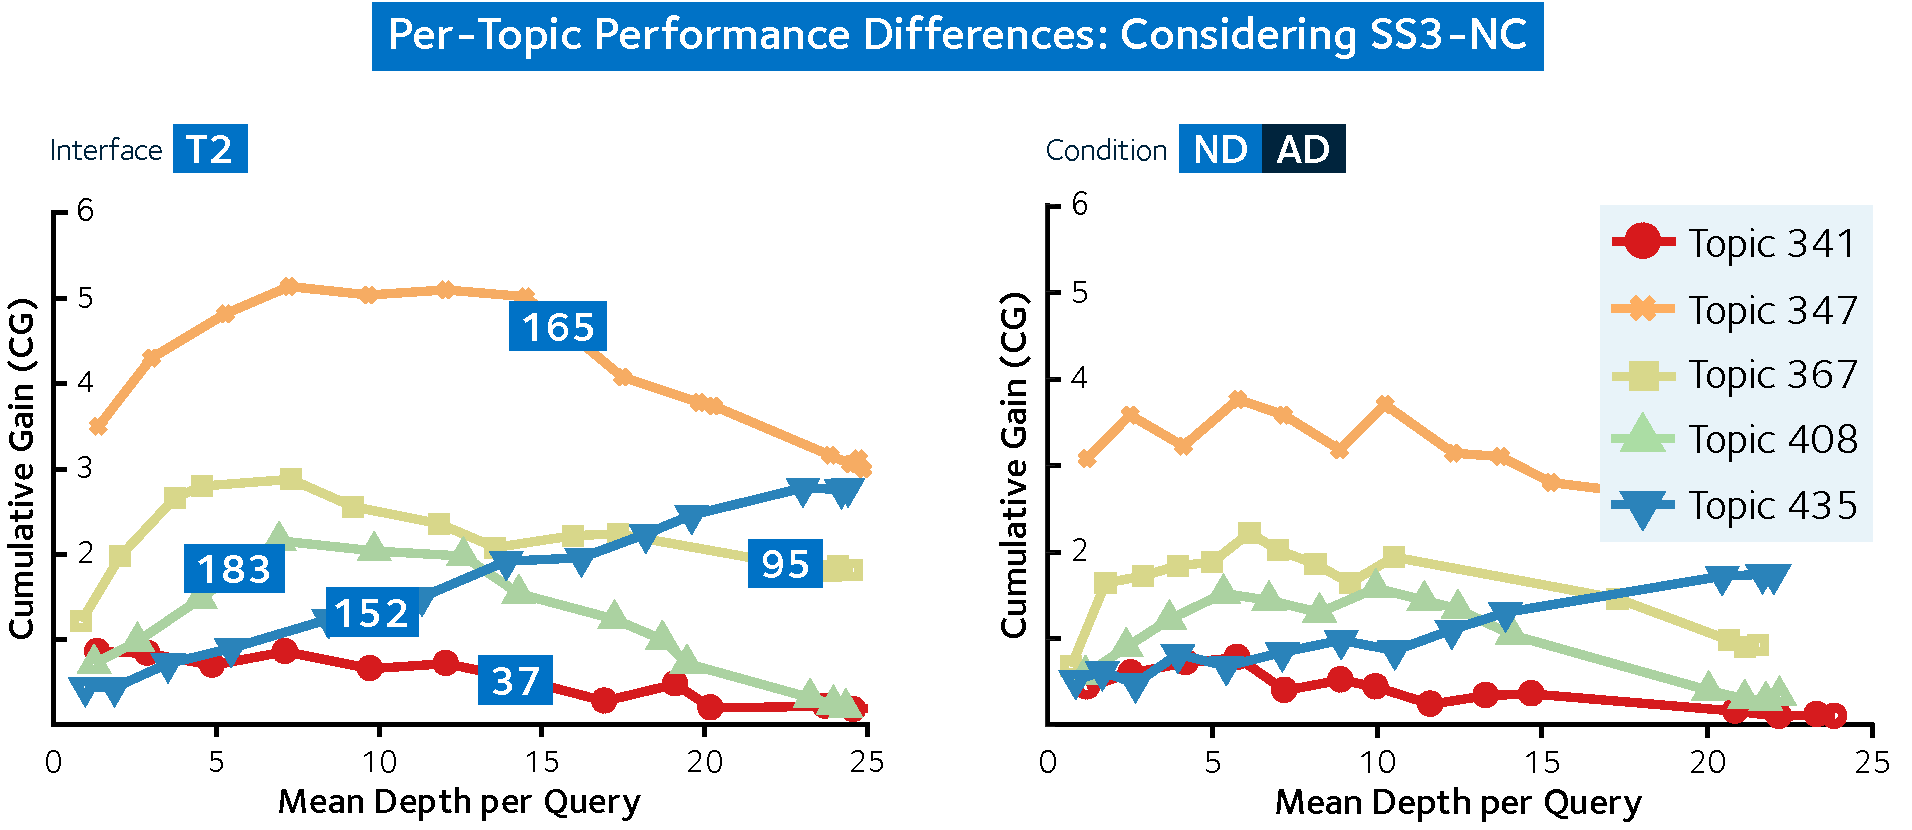
\includegraphics{figures/ch10-per_topic.pdf}}
    \caption[Per-topic performance variation example]{Plots demonstrating the wide per-topic variance over the \emph{what-if} performance simulations. On the left, performance over interface \blueboxbold{T2} is shown \textemdash~\dualbluebox{ND}{AD} is shown on the right. Stopping strategy \blueboxbold{SS3-NC} is used for this demonstration. Similar observations were observed across other interfaces, conditions and stopping strategies. Also \blueboxbold{highlighted} on the left plot is the number of~\gls{acr:trec} relevant documents for each topic. Note the general performance improvement as the number of~\gls{acr:trec} relevant documents increases for a topic.}
    \label{fig:per_topic_differences}
\end{figure}

Considering point~\raisebox{-.2\height}{
\includegraphics[height=5mm]{figures/ch2-point1.pdf}} first, we note that the same gain stopping threshold values were trialled over all five topics in the reported simulations of interaction. Table~\ref{tbl:ch6_topic_rels} on page~\pageref{tbl:ch6_topic_rels} demonstrated that the number of~\gls{acr:trec} relevant documents for each of the five topics varies considerably. As such, one would expect that the computed rate of gain would also vary considerably on a per-topic basis. This way, expectations of gain can be kept in check -- a rate of gain threshold computed over a performant~\gls{acr:trec} topic with many relevant documents would perform much worse under a topic for which it is much harder to find relevant documents for (i.e. a comparatively smaller number of~\gls{acr:trec} relevant documents). This variation in the number of relevant documents over topics (amongst other factors, such as the retrieval system used) is illustrated in Figure~\ref{fig:per_topic_differences}. Using interface \blueboxbold{T2} (left) and condition \dualbluebox{ND}{AD} (right) over \blueboxbold{SS3-NC}, the two plots in the figure illustrate the variation in performance across the five topics trialled. We also note a general trend of higher performance for a topic in the plots if a greater number of~\gls{acr:trec} relevant documents are present.

We also consider how the rate of gain is computed, as per point~\raisebox{-.2\height}{
\includegraphics[height=5mm]{figures/ch2-point2.pdf}}. \emph{How do searchers estimate a rate of gain threshold?} This is a difficult question to answer, with further study required to address this. However, one would be pressed to believe that from an initial impression of a~\gls{acr:serp}, a searcher would undertake a series of computations in their head to reach an estimation for a rate of gain threshold value. It is much easier to believe that searchers would rather employ a simpler stopping criterion in this instance, such as \emph{stopping after observing $k$ non-relevant result summaries} (i.e. the frustration-based heuristic). This can be simplified with the example of an individual throwing a ball in the air. It would be easier to believe that the ball thrower would think of how to catch the ball in relation to how it is falling through the air, with feedback from their visual and proprioception systems. This is opposed to believing that the thrower of the ball may catch it by calculating the equations of the underlying physics of the falling ball to predict the optimal point in space at which to catch it.

However, even if we were able to provide better values for the rate of gain, would we see improvements in real-world approximations? While~\gls{acr:ift} says that we will, individuals may be behaving in a suboptimal way. A body of literature in ecology suggests that when foraging for food in the wild, animals \emph{do} behave in a suboptimal way.~\cite{janetos1981imperfectly} and~\cite{krebs1983perspectives} state that animals may employ some \emph{rule of thumb} that is less than perfect, with an example cited as \emph{`take the largest thing you can eat'.} This is some ways analogous to the more simplistic stopping strategies we trialled.~\cite{krebs1983perspectives} also argue that these simplistic approaches are actually an optimisation within a wide number of constraints, such as sensory limitations. This may be true of searchers, too -- with limited working memory, a more simplistic approach may, in reality, be the better, optimal choice even though the theory may suggest otherwise.

\blueboxheader{\gls{acr:rbp} Stopping Strategy}
We also observed that \blueboxbold{SS12-RBP}, the~\gls{acr:rbp}-based stopping strategy, also generally failed to provide a good approximation. Performance in the \emph{what-if} simulations was generally significantly different from the best performing stopping strategies, although instances such as \blueboxbold{T2} did not demonstrate any significant difference. While performance matchups might have been relatively good, the depths to which simulated searchers examined content using this stopping strategy were weak to a considerable degree. Refer to plot \blueboxbold{SS12-RBP} in Figure~\ref{fig:ch7_sim_comparison_plots} on page~\pageref{fig:ch7_sim_comparison_plots} for an example.) Recall the patience parameter $p$ of~\gls{acr:rbp}, that dictated how deep down a list of ranked results a searcher would be prepared to go. The point at which the searcher would decide to stop was modelled stochastically. In the real-world, searchers do not roll a dice to determine when to stop, but rather rely upon some form of an intuitive informational cue, as have been previously shown to affect search behaviours.

\blueboxheader{Considering more Performant Stopping Strategies}
Combination-based stopping strategies \blueboxbold{SS5-COMB} and \blueboxbold{SS11-COMB} both performed and approximated stopping behaviours well. Formed of more simplistic stopping strategies (e.g. \blueboxbold{SS2-NT}), results seem to suggest that searchers do not consider a single criterion when determining the point at which they should stop examining results -- an intuitive finding.

This interesting conclusion can be corroborated by other recent studies. Work by~\cite{zhang2017bejewled} used the \emph{Bejeweled Player Model (BPM)} to model a searcher's stopping behaviours, where they would stop when:

\begin{quote}
    \emph{``he/she either has found sufficient useful information, or no more patience to continue.''}
    \attrib{\cite{zhang2017bejewled}}
\end{quote}

Findings from this study demonstrated improvements in the correlations between searcher satisfaction and existing~\gls{acr:ir} evaluation measures. This was also corroborated in a recent study by~\cite{azzopardi2018cwl}. Central to this argument is the similarity of the BPM to \blueboxbold{SS5-COMB}, that considered a combination of the satiation (\blueboxbold{SS4-SAT}) and frustration (\blueboxbold{SS2-NT}) stopping strategies. This provides evidence that empirically validates the inclusion of both satiation and frustration-based stopping heuristics within the searcher model. The evidence is clearly showing that multiple criteria are being considered when a stopping point is decided, and future work should consider the development of measures that support both criteria.

Overall, a majority of stopping strategies performed well and produced approximations that were very close to one another, with few significant differences. One particularly surprising result was that of \blueboxbold{SS1-FIX}. The fixed-depth, non-adaptive baseline approach consistently offered good performance and approximations. This is counter-intuitive, as it would make sense for more adaptive strategies to offer improved approximations. It is likely that different subjects would have employed different stopping strategies, or a variety of different strategies depending upon the situation (i.e. as demonstrated by \blueboxbold{SS11-COMB}). In this regard, next steps should consider stopping behaviours on an individual level. However, from the perspective of averaging over a population, many of the stopping strategies trialled, when tuned appropriately (i.e. \dualbluebox{SS1-FIX}{@24}, which one could argue as being wholly unrealistic), offer good approximations and performance.

\subsection{Searcher Behaviours}\label{sec:conclusions:discussion:behaviours}
From the reported user studies, it is clear that the interfaces and conditions that we trialled do affect the behaviours of searchers. In terms of stopping behaviours, we did observe differences, but differences often were not significant. We hypothesise that due to the high levels of variance that we observed, larger sample sizes over each study would be required in order to tease out significant differences and to provide data for further examination.

Understanding stopping behaviours is a difficult challenge. What findings from our studies do suggest is that variations in interfaces, tasks, goals and systems do impact upon performance. For example, as we increased result summary lengths, stopping depths became shallower (i.e. from \blueboxbold{T0}$\rightarrow$\blueboxbold{T4}). More extreme interfaces and conditions would likely amplify the effect we observe. Factors such as how the prior topic knowledge that a subject possesses were also not considered in this thesis, and would likely play a role in stopping behaviours. We leave this to future work.

\subsection{Simulations of Interaction}\label{sec:conclusions:discussion:simulations}
In this thesis, we have presented significant advancements in terms of modelling and understanding the~\gls{acr:iir} process. We developed an extensive framework that allowed us to change components of the underlying~\gls{acr:csm}. Given this framework, we could then formulate the search problem more precisely, and explore the impact that each of the component variations had on the wider search process. As components were changed, we were able to demonstrate improvements in the approximations of human searcher behaviours. Given the limitations of our user studies with potentially insufficient data, simulations of interaction allowed us to generate more data at a much lower cost.

One particularly novel contribution concerning the simulations of interaction was addressing the issue of comparing results across different configurations. Being stochastic in nature, the simulations relied upon the roll of a dice to determine whether a simulated searcher would click on a result summary link (if deemed sufficiently attractive to warrant further examination), or save a document as relevant (if deemed relevant to the given information need). These were grounded on the~\gls{acr:trec} relevance judgements and interaction probabilities extracted from the user studies. Across different configurations however, outcomes of the dice roll would have resulted in different decisions being taken -- which in turn ensured that when examining two configurations, their outcomes would not be comparable.

Section~\ref{sec:method:simulation:grounding:judgements} on page~\pageref{sec:method:simulation:grounding:judgements} outlined a \emph{pre-rolled judgements} technique that rolled the dice \emph{a priori} 50 times, with 50 being the number of trials that were run per configuration. This then meant that during the simulations, the decision maker components of the \simiir~framework essentially became deterministic, extracting the judgement for a particular trial from a pre-rolled \emph{action judgement file.} In turn, this addressed the issue of comparability between different configurations. With the same judgements, comparisons became fairer. Of course, a larger number of trials would always be desirable as a means of teasing out further differences that perhaps would otherwise not have been observed.

We also note limitations of the approach taken in conducting our simulations of interaction. Most notably, we considered the \emph{most optimistic outcome} at several points in our simulations, mostly pertaining to the perceived quality of a~\gls{acr:serp}. A prime example of this was highlighted in Section~\ref{sec:conclusions:discussion:realism}, with the \blueboxbold{Perfect}~\gls{acr:serp} level stopping decision point implementation discussed as the implementation yielding significant improvements in performance, yet attaining this with access to~\gls{acr:trec} QREL judgements.

A further example of this approach was demonstrated with combination stopping strategy \blueboxbold{SS11-COMB}. Similar to the~\gls{acr:serp} level stopping decision point, this strategy took an initial impression of a presented~\gls{acr:serp}, and used this impression to select an appropriate constituent stopping strategy -- with either \blueboxbold{SS4-SAT} for a~\gls{acr:serp} yielding relevant documents early in the rankings, or \blueboxbold{SS10-RELTIME} for a~\gls{acr:serp} of dubious quality. Under these conditions, such strategies do intuitively make sense. However, the decision was again made with access to~\gls{acr:trec} QRELs -- $P@1$ was used to determine if the~\gls{acr:serp} yielded relevant content at shallow ranks. If, for example, a stochastic approach were to be implemented in determining what stopping strategy to employ, it may mean that even better approximations could be achieved.

\section{Future Research Directions}\label{sec:conclusions:future}
From the summary and discussion of our empirical results, a number of potential avenues for future work may be considered. In this section, we consider: how to improve the realism of simulations of interaction further; stopping heuristics and strategies; simulation trials and topics; and the modelling of stopping from the level of individual searchers.

\subsection{Improving Simulation Realism}\label{sec:conclusions:future:improving}
In this thesis, we presented the~\gls{acr:csm}, a high-level, conceptual searcher model. It encapsulates many of the different activities and decision points that searchers would contend with across informational search tasks. With the inclusion of the new~\gls{acr:serp} level stopping decision point, improvements were made to the realism of the simulations that were executed with the~\gls{acr:csm}. However, \emph{what changes could we subsequently make to the~\gls{acr:csm} and related infrastructure in future work that would aid in advancing the realism of these simulations further?} As illustrated below, we consider this open question from three main research strands.

\begin{figure}[h!]
    \centering
    \resizebox{1\hsize}{!}{
    
\includegraphics[width=1\textwidth]{figures/ch10-future_simulations.pdf}}
\end{figure}

\blueboxheader{Contextual and Cognitive}
Our first strand considers \genericblack{contextual} and \genericblack{cognitive} factors. All experimentation in this thesis was conducted under the domain of news search, with subjects of the user studies asked to imagine that they were newspaper reporters, having being given a task to find documents that they thought were relevant to a particular topic. However, this scenario is very specific. If we performed studies with the same methodology, but under a different search context, would we find similar results? Arguably, behaviours will change -- general web search and a detailed examination of content under the context we employed will result in different outcomes. Different tasks can also be considered. Aspectual and ad-hoc tasks were considered as we believed they would offer the greatest difference in terms of stopping behaviours. Would other retrieval tasks offer even bigger differences in terms of searcher behaviours?

Other factors such as the location at which the search is undertaken, the device upon which the search is undertaken and other external pressures will also undoubtedly influence the outcome of the results obtained. Crowdsourced subjects whose behaviours are reported in this thesis conducted our experiments on a desktop or laptop computer. They were instructed to be in a comfortable, quiet location, free from major distractions. In reality, individuals are less likely to search in such conditions. Perhaps time pressures would influence their behaviours -- a student under pressure to finish a draft of her paper will behave differently to one who is not under the same pressure. With the proliferation of mobile devices such as smartphones, searching on such devices must also be considered. A recent study by~\cite{ong2017scent_behaviour} demonstrated that search behaviours, for example, do differ between individuals using desktop computers and smartphones.

Much work remains to determine how we can try to understand and subsequently model the cognitive processes and factors that influence how individuals behave when searching. Individuals are products of their prior experiences, and are therefore unique; behaviours will undoubtedly differ from person to person. Within the modelling process, novel techniques can be applied that could possibly improve the realism of simulations. For example, within the \simiir~framework, the search context component tracks a list of queries issued, documents examined (and saved), along with other measures. Could this component be manipulated in such a way as to better mimic the behaviours of a human? Rather than maintaining a perfect list of everything that has been examined, a simulated searcher could be programmed to become `forgetful' in remembering what they have examined, with certain cues within a document reminding them that this is something that they may have previously examined. Other factors, such as prior topic knowledge (as alluded to in Section~\ref{sec:conclusions:discussion:behaviours}) ought to be considered, as such aspects would likely impact upon the stopping behaviours of searchers.

As alluded to in Chapter~\ref{chap:diversity}, further work could also be undertaken in relation to the decision maker components of the \simiir~framework. This work would consider how simulated searchers would judge the attractiveness of result summaries and relevancy of documents to a given topic. Decision makers were implemented primarily with ad-hoc retrieval in mind, considering only the probability of clicking or saving with respect to the~\gls{acr:trec}~\gls{acr:qrel} judgement. For aspectual retrieval tasks, further work would consider whether the result summary or document contains a discussion of new entities for the topic, such as a previously unseen species of animal.

\blueboxheader{Conceptual Modelling}
We next consider a number of further enhancements to the~\gls{acr:csm} that could improve the realism of simulations further. Examples in the illustration above consider potential areas for future improvement. \genericblack{Tool switching}, as demonstrated by~\cite{thomas2014modelling_behaviour}, would be considered at the beginning of the search process. It would enable a searcher to determine what tool, or retrieval system, would be better suited to help them satisfy their information need. This is opposed to the current~\gls{acr:csm} as presented in the thesis, that assumes a retrieval system has been selected \emph{a priori.} A study by~\cite{white2009tool_switching} has shown that predicting tool switching is feasible. They reported that sufficiently consistent behaviours exhibited by searchers in relation to this phenomenon led to accurate predictions of tool switching events.

\genericblack{Results pagination} is also listed in the illustration above. Here, a simulated searcher will be presented with~\glsplural{acr:serp} that are split across a number of different pages, rather than examining a continuous ranked list of results. This would involve the notion of extracting additional grounding data from interaction logs, perhaps such as the likelihood of a searcher continuing to the next~\gls{acr:serp} page. This would likely impact upon the realism of simulations, as a study by~\cite{jansen2005analysis} showed a sharp decrease in content examined after the first page of results. Further examination of modelling stopping behaviours within the~\gls{acr:csm} is also considered; refer to Section~\ref{sec:conclusions:future:stopping} for further details.

\blueboxheader{Stochastic to Deterministic} Decisions pertaining to the attractiveness of result summaries and the relevance of documents within our simulations of interaction were determined \emph{stochastically,} or by a roll of the dice. While a simplifying assumption that has been used in many other studies employing simulations of interaction, this is an unrealistic approach. If implemented correctly, a more \emph{deterministic} solution would offer more realistic simulations, where simulated searchers would be able to \emph{learn} as they traverse through content, improving their decision making abilities based upon the content observed, rather than the outcome of a roll of a dice. Advancements in understanding the \emph{information triage} process would undoubtedly lead to improved realism. In addition, the inclusion of \emph{variable interaction costs} would also benefit the realism of future simulations.\footnote{As discussed previously in this thesis, \emph{time-biased gain}~\citep{smucker2012tbg} is an example of such an approach.}

\subsection{Stopping Heuristics and Strategies}\label{sec:conclusions:future:stopping}
In this thesis, we considered a total of twelve different stopping strategies, operationalised from a total of eight different stopping heuristics (and the~\gls{acr:rbp}~\gls{acr:ir} evaluation measure). We showed how each of the different strategies perform over a number of different experimental interfaces and conditions. During the methodological design stage, it became apparent that the approaches taken for the operationalisation of the selected stopping strategies were just one of many. \emph{What if we implemented our stopping strategies in different ways? Why did we select these strategies?} Here, we consider these questions with insight into what might happen if they were to be explored further.

\blueboxbold{Stopping Decision Points}
Following on with the theme of improving the underlying~\gls{acr:csm}, additional stopping decision points could be included. These would provide searchers subscribing to the~\gls{acr:csm} with greater flexibility regarding when they stop examining content. Additional stopping decision points could, for example, include one for tool switching. In this example, a searcher, after spending some period of time on one retrieval system, could decide to stop using it after certain criteria are met. After this point has been reached, they will then switch to a different retrieval system. A further interesting research question would be whether the result summary level stopping strategies trialled in this thesis would work at different stopping decision points. For example, at a session level, would these strategies make sense? Would using them at that decision point lead to a better matchup with real-world stopping behaviours?

\blueboxbold{Stopping Strategy Selection}
From here, we can also consider a further decision point that could be encoded within the~\gls{acr:csm}. Inspired by \blueboxbold{SS11-COMB}, consideration must be taken into deciding \emph{why} and \emph{when} a particular stopping strategy could be employed. As we demonstrated in Figure~\ref{fig:ss11_combo} on page~\pageref{fig:ss11_combo}, \blueboxbold{SS11-COMB} employs both the frustration and give-up time-based stopping heuristics -- but not at once. Rather, a decision is made pertaining to the quality of the presented~\gls{acr:serp} (much like the~\gls{acr:serp} level stopping decision point). The outcome of this decision then dictates what stopping strategy is employed for the remainder of the query. Further refinements to this approach could, for example, include additional stopping strategies and a wider range of conditions for employing them. Empirical evidence could be extracted from interaction logs to determine if, under certain circumstances, searchers would favour one approach over another.

\blueboxbold{Stopping Strategy Operationalisation}
An open question arising from the work in this thesis considers: \emph{how do you operationalise the stopping heuristics?} Clearly, from the outline of the twelve stopping strategies in Chapter~\ref{chap:strategies} on page~\pageref{chap:strategies} (and implementation methodology in Section~\ref{sec:method:simulation:grounding:stopping} on page~\pageref{sec:method:simulation:grounding:stopping}), there are a large number of different ways in which the stopping strategies can be implemented. While we provided a means and justification for the approaches that we took in this thesis, we have reason to believe that some of the stopping strategies -- especially \blueboxbold{SS6-DT}, \blueboxbold{SS7-DKL} and \blueboxbold{SS8-IFT} -- performed poorly, perhaps because of our implementations (refer to Section~\ref{sec:conclusions:discussion:strategies}). For example, the rate of gain for \blueboxbold{SS8-IFT} could have been computed on a per topic basis. Further work will be required in order to determine if different implementations would lead to performance improvements.

\blueboxbold{Considering Additional Stopping Heuristics}
Of course, the eight stopping heuristics that we considered in this thesis do not constitute the entirety of the heuristics defined in the literature. We selected these heuristics as they offered interesting differences between one another, were \emph{relatively} straightforward to implement, and would likely be discernible across complex informational search tasks (although this was not necessarily proved). Unused heuristics such as the mental list stopping heuristic (considering different criteria that must be met, as outlined by~\cite{nickles1995judgment} and detailed in Section~\ref{sec:stopping_background:heuristics:mental} on page~\pageref{sec:stopping_background:heuristics:mental}) would have been much more challenging to operationalise and implement -- and even so, would such a heuristic be suitable for the task at hand? The ability for a searcher to create a series of bullet points about a topic would imply he or she has some sound idea of their objective. The searcher's knowledge of a topic may be so limited that such a heuristic would be unsuitable. Linking back to contextual factors above, considering additional search contexts (perhaps with searchers of astute and limited knowledge of a topic) would be interesting to examine.

\blueboxbold{Towards Future~\gls{acr:ir} Measures}
Given the above, findings from this research provide motivation for further work considering the inclusion of stopping heuristics within the measures that are used within~\gls{acr:ir} research. For example, stopping strategy \blueboxbold{SS5-COMB} demonstrated good overall and performance considering a searcher's satisfaction and tolerance toward non-relevant material. This has also been shown in the BPM~\citep{zhang2017bejewled}.

\subsection{Simulation Trials and Topics}\label{sec:conclusions:future:running}
We also consider future work in terms of \emph{how} the simulations of interaction could be run. While 50 trials were selected because of the fact that approximately 50 subjects partook in each user study, there are likely trends and significant differences that exist that we simply did not observe because of a lack of experimental power. This limitation was also imposed with an insufficient amount of processing power to complete the experiments in a reasonable timeframe.\footnote{Using the experimental setup detailed in this thesis, all simulations of interaction took approximately $38$ days of processing time.} With more powerful computer hardware, scaling up the experiments with more trials would have become a more realistic prospect.

We also consider using five topics for our performance \emph{(what-if)} experiments to be a limiting factor. While the decision to use five topics was justified due to a lack of data (considering entities across the remaining 45 topics in Chapter~\ref{chap:diversity}) -- and to ensure that comparisons between interfaces and conditions were fair -- 50 topics would have been preferred (refer to Figure~\ref{fig:per_topic_differences}). If (aspectual) data were available for the remaining 45 topics, we could then trial additional performance runs, which may also lead to the observation of other trends and potential significant differences.

\subsection{Individual Searcher Stopping Behaviours}
Our final consideration for future work revolves around the notion of \emph{individual searcher stopping behaviours.} In this thesis, we considered searcher stopping behaviours, reported across $\approx50$ subjects, over each interface and condition that was trialled. This provided us with a rough approximation as to what strategies work best, with similar findings reported across interfaces and conditions. However, research has shown that individual searcher behaviours may differ to a significant degree. If we considered individual searchers, what trends would we then observe? Examining behaviours on a per-searcher level will avoid the watering down of results through averaging over a particular cohort, exposing more interesting results. For example, could we perform a classification of searcher stopping behaviours? Such an approach was followed, for example, by~\cite{smucker2011user_strategies}, who devised a classification of searchers when examining documents -- with searchers being categorised into one of either \emph{fast and liberal} or \emph{slow and neutral}. This is undoubtedly one key area of future work that we must consider in order to develop a deeper understanding of the stopping behaviours that searchers employ.

\section{Final Remarks}\label{sec:conclusions:remarks}
Stopping during the search process is a difficult phenomenon to understand and model effectively. A wide range of different factors influence the internal decision-making process of searchers. We have shown in this thesis that a number of simplistic stopping strategies can offer improved performance and approximations of real-world searcher behaviours. We also provide novel evidence to motivate the fact that multiple stopping criteria need to be considered in the development of future~\gls{acr:ir} evaluation measures, along with the inclusion of additional stopping decision points to improve the realism of future searcher models. The development of the~\gls{acr:csm} has also been positive, with a solid baseline provided for future work in developing ever more realistic simulations of interaction.

Despite the inherently difficult task that understanding and modelling stopping behaviours represent, we believe that the potential benefits of further exploration in this area will undoubtedly aid the searchers and researchers of future retrieval systems. Now that this is all done, \emph{I} am off to the pub -- and having reached the end of this thesis, you should go, too!

% \newpage
% \thispagestyle{empty}
% \mbox{}
% \newpage
% \thispagestyle{empty}
% \mbox{}
% \newpage